% !TEX root =  ../main.tex 

\section{Simulation study}
\label{sec: simulation_study}
The application of personalized schedules for patients from PRIAS program demonstrated that personalized schedules adapt according to the PSA and repeat biopsy history of each patient. However, the patients in PRIAS have already had their biopsies as per the PRIAS schedule, and hence evaluation of the efficacy of personalized schedules against the PRIAS schedule was not possible. To this end, we have performed a simulation study to compare 3 broad categories of schedules: Personalized schedules, PRIAS schedule and annual schedule. To compare the schedules we employ them for simulated patients enrolled in a hypothetical AS program, with the same entrance criteria as PRIAS. For these patients we simulate the evolution of PSA and the time of GR. Since our interest is only in the schedule of biopsies, we keep a fixed schedule for PSA measurements. The hypothetical repeat biopsies are conducted till the GR is detected. Although Gleason scores are susceptible to inter-obserer variation \citep{Gleason_interobs_var}, we assume that any biopsy conducted after the true GR time of a patient will lead to GR detection with 100\% certainty. We next present the details of the simulation study and the biopsy schedule evaluation criteria.

\subsection{Simulation setup}
\label{subsec : simulation_setup}
\subsubsection{Patient population}
For the simulation study we first select a population $\mathcal{P}$ of patients enrolled in AS. We assume that the PSA and hazard of GR for the patients from this population follows a joint model of the form postulated in Section \ref{subsec : jm_fit_prias}, with parameters $\boldsymbol{\theta}^{\mathcal{P}}$. These parameters are selected to be equal to the posterior mean of parameters $E[\boldsymbol{\theta} \mid \mathcal{D}^{PRIAS}]$ estimated from the joint model fitted to PRIAS data set (Section \ref{subsec : param_estimates_jm_fit_prias}). To demonstrate the efficacy of personalized schedules for patients with early as well late failure times, we generated the patients in population $\mathcal{P}$ from 3 equal sized sub-groups. The baseline hazard for each of the sub-group was assumed to be the hazard function of a Weibull distribution. The shape and scale parameters $(k, \lambda$) for this Weibull distribution are $(1.5, 4)$, $(3, 5)$ and $(4.5, 6)$.

\subsubsection{Generating PSA values and GR times}
From the population $\mathcal{P}$ we randomly sample a total of 200 data sets with 1000 patients each. For each of these patients, the longitudinal profiles for PSA In terms of average number of biopsies, the PRIAS schedule, schedules based on dynamic risk of GR and annual schedule are quite similar. However the dynamic risk of GR based schedules have much lower corresponding variance. In general we observe that there is an inverse relationship between offset number of biopsies.\\
s are generated as per the visiting schedule of PRIAS study. i.e. Every 3 months for first 2 years and every 6 months thereafter. The true GR times are generated as per the simulated hazard of GR for the patient. We then divide each of the 200 simulated data sets into training (750 patients) and test (250 patients) parts. Keeping in line with the notation for joint model in Section \ref{subsec : jm_specification}, the observed data in the $k^{th}$ training data set can be represented as $\mathcal{D}^k = \{l_{ki}, r_{ki}, \boldsymbol{y}_{ki}; i = 1,\ldots 750\}$, where $\boldsymbol{y}_{ki}$ denotes the PSA measurements for the $i^{th}$ patient in the $k^{th}$ training data set. For training data patients we either observe the true event time $T^*_{ki}$, wherein $l_{ki} = r_{ki} = T^*_{ki}$, or we observe a random and non-informative censoring time $C_{ki} < T^*_{ki}$, wherein $l_{ki} = C_{ki}$ and $r_{ki} = \infty$. For the patients in the test data sets no censoring times are generated.

\subsubsection{Personalized schedules for test patients}
\label{subsubsec : sim_study_pers_sched_details}
We create personalized biopsy schedules only for the patients in the test data set. To this end we first fit a joint model with the same specification as for PRIAS (Equation (\ref{eq : long_model_prias}) and (\ref{eq : hazard_prias})). to the training data set. To model the baseline hazard we use a P-splines approach (Section \ref{subsec : jm_specification}). From the fitted joint model we obtain posterior distribution of parameters $p(\boldsymbol{\theta} \mid \mathcal{D}^k)$, which is required for the posterior predictive distribution $g(T^*_{kj})$ of the $j^{th}$ test patient from the $k^{th}$ data set. While the posterior predictive distribution is sufficient for scheduling biopsies based on expected time of GR, the choice of time window $\Delta t$ (Section \ref{subsubsec : dynamic_risk_definitions}) has to be made for scheduling biopsies on the basis of dynamic risk of GR. In PRIAS and in most AS programs biopsies are done at a gap of 1 to 3 years. A gap of 1 year between biopsies detects GR the earliest, and in worst case the detection of GR can be delayed by 1 year. Being a clinically relevant period of time to differentiate between patients who obtain GR and those who don't, we choose a $\Delta t$ of 1 year. Further, in schedules based on dynamic risk of GR, for a test patient $j$, we choose a value of $\kappa$ which maximizes a binary classification measure (Section \ref{subsubsec : kappa_estimation}) at the last known repeat biopsy time $t$ of the patient. To this end the binary classification measures are first computed over a fine grid of $\kappa$ values in the interval $[0,1]$ using the training data set and then the most optimal $\kappa$ is chosen.\\

To create personalized schedules we employ the algorithm described in Section \ref{subsec : pers_sched_algorithm}. The algorithm is run for 7 different settings, one each corresponding to the following: PRIAS schedule, annual schedule, expected time of GR, median time of GR, dynamic risk of GR with $\kappa$ chosen such that a) Youden's $J$ is maximized, b) $\text{F}_1$-Score is maximized. In addition to these a mixed approach (Section \ref{subsec : mixed_approach}) is also employed where a choice between median time of GR and dynamic risk of GR (Youden's $J$ maximized) is made before scheduling a biopsy.

\subsection{Evaluating efficacy of scheduling methods}
For a particular biopsy scheduling method $S$, the first criteria in the evaluation of efficacy of the method is the number of repeat biopsies $N^{bS}$ the corresponding schedule takes before GR is detected for a patient from the population. As we discussed earlier, the less the $N^{bS}$ the better it is for the patients. Our interest lies in the marginal distribution of $N^{bS}$ for the population $\mathcal{P}$. In its simplest form, the mean $E[N^{bS}]$ and variance $Var[N^{bS}]$ of the aforementioned distribution are indicators of the performance of the scheduling algorithm. More specifically, a low mean as well as low variance is desired. Other quantiles of the distribution may also be used evaluation criteria. For e.g. a method which takes less than 2 (say) biopsies in 95\% cases may be preferred.\\

The second criteria in evaluation of efficacy of a schedule is the offset. Given a scheduling method $S$, the offset for a particular patient $j$ is defined as $O^S_j = T^S_{j{N^{bS}_j}} - T^*_j$, where $N^{bS}_j$ is the number of biopsies required for patient $j$ before GR is detected and $T^S_{j{N^{bS}_j}} > T^*_j$ is the time at which GR is detected by the scheduling method $S$. Once again the interest lies in both the mean $E[O^S]$ and variance $Var[O^S]$ of the marginal distribution of offset.

\subsubsection{Finding the most optimal schedule}
Given the multiple criteria for efficacy of a schedule the next step is to find the most optimal schedule. Using principles from compound optimal designs \citep{lauter1976optimal} we propose to choose a scheduling method $S$ which minimizes the following loss function:

\begin{equation}
\label{eq : loss_func_sim_study_generic}
L(S) = \sum_{g=1}^G \lambda_g \mathcal{G}_g(N^{bS})^{d_g=1}\mathcal{G}_g(O^S)^{d_g=0}
\end{equation}
where $\mathcal{G}_g(\cdot)$ is either a function of number of biopsies or of the offset, and $d_g$ is the corresponding indicator for this choice. Some examples of $\mathcal{G}_g(\cdot)$ are mean, median, variance and quantile function. Constants $\lambda_1, \ldots \lambda_G$, where $\lambda_g \epsilon [0,1]$ and $\sum_{g=1}^G \lambda_g = 1$, are weights to differentially weigh-in the contribution of each of the $G$ evaluation criteria manifested via the functions $\mathcal{G}_g(\cdot)$. An example loss function is:

\begin{equation}
\label{eq : loss_func_sim_study}
L(S) = \lambda_1 E[N^{bS}] + \lambda_2 E[O^S] 
\end{equation}
The choice of $\lambda_1$ and $\lambda_2$ is not easy. This because biopsies have serious medical side effects and the cost of an extra biopsy cannot be quantified easily. To obviate this issue we utilize the equivalence between compound and constrained optimal designs \citep{cook1994equivalence}. More specifically, it can be shown that for any $\lambda_1$ and $\lambda_2$ there exists a constant $C>0$ for which minimization of loss function in Equation (\ref{eq : loss_func_sim_study}) is equivalent to minimization of the same, subject to the constraint that $E[O^S] < C$. i.e. The optimal schedule is the one with the least number of biopsies and an offset less than $C$. The choice of $C$ now can be based on the protocol of AS program. For e.g. in PRIAS the maximum gap between 2 repeat biopsies is 3 years. i.e. If GR is detected within 3 years of its occurrence, it is acceptable. The optimization in case of more than 2 criteria, such as in Equation (\ref{eq : loss_func_sim_study_generic}), the solution can be found by minimizing $\mathcal{G}_G(\cdot)$ under the constraint $\mathcal{G}_g < C_g; g=1, \ldots G-1$.\\

For the loss function in Equation (\ref{eq : loss_func_sim_study}), we estimate $E[N^{bS}]$, $Var[N^{bS}]$, $E[O^S]$ and $Var[O^S]$ using pooled estimates of each from the 200 repetitions of the simulation study. The estimates are calculated separately for each of the 7 methods mentioned in Section \ref{subsubsec : sim_study_pers_sched_details}. The pooled estimates for a scheduling method $S$ are calculated as following:

\begin{align*}
\widehat{E[O^S]} &= \frac{\sum_{k=1}^{200} n_k \widehat{E[O^S_k]}}{\sum_{k=1}^{200} n_k}, \\
\widehat{Var[O^S]} &= \frac{\sum_{k=1}^{200} (n_k - 1) \widehat{Var[O^S_k]}}{\sum_{k=1}^{200} (n_k-1)}, 
\end{align*}
where $n_k$ are the number of test patients in the $k^{th}$ simulation, $\widehat{E[O^S_k]} = \frac{\sum_{j=1}^{n_k}O^S_{kj}}{n_k}$ and $\widehat{Var[O^S_k]} = \frac{\sum_{j=1}^{n_k}(O^S_{kj} - \widehat{E[O^S_k]})^2}{n_k-1}$ are the estimated mean offset and estimated variance of the offset for the $k^{th}$ simulation, respectively. The estimates for number of biopsies $N^{bS}$ are calculated similarly.

\subsection{Results}
From the simulations we calculated the pooled estimates of the mean and variance of number of biopsies, and the same for the offset. They are summarized in Table \ref{table : sim_study_pooled_estimates} and Figure \ref{fig : meanNbVsOffset}. The annual schedule has the least estimated $E[O^S]$, of 6 months, and also the least $Var[O^S]$ among all the methods. The downside of the method is that it has the largest estimated $Var[N^{bS}]$, with $E[N^{bS}]$ being 5.2. If we compare it to the schedule based on expected time of GR, the $Var[N^{bS}]$ is almost 4.6 times less and on average 1.9 biopsies are scheduled before GR is detected. This however comes at a cost of having larger offsets. Expected time of GR and median time of GR, both have the highest $E[O^S]$ of around 15.1 and 13.9 months respectively. They also have the highest $Var[O^S]$. Thus there is an inverse relationship between offset and number of biopsies.\\

\begin{figure}[!htb]
	\centering
    \captionsetup{justification=centering}
	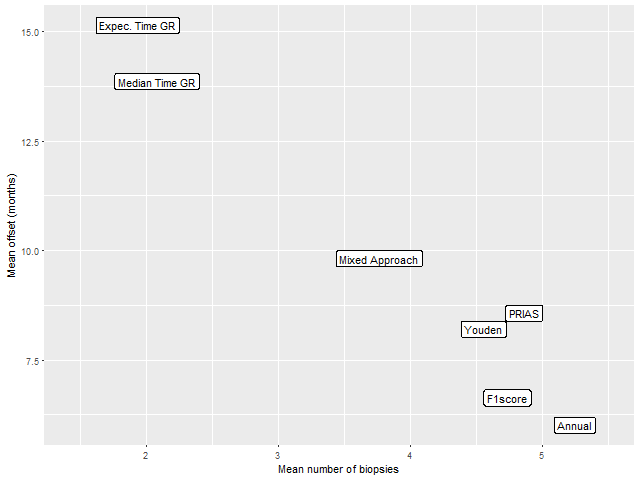
\includegraphics[width=0.8\textwidth]{images/sim_study/meanNbVsOffset.png}
	\caption{Estimated mean number of biopsies and mean offset (months) for the 7 scheduling methods. Method names are abbreviated for ease of graphing.}
	\label{fig : meanNbVsOffset}
\end{figure}

If we compare the PRIAS schedule and annual schedule the latter may be preferred since it offers the least $Var[O^S]$ and $E[O^S]$ while its $E[N^{bS}]$ and $Var[N^{bS}]$ are quite similar to that of PRIAS schedule. If we compare the PRIAS schedule with dynamic risk of GR based schedules, we can see that the schedule where $\kappa$ is chosen after maximizing $\text{F}_1$-Score, performs better than in PRIAS schedule in all aspects. The schedule where $\kappa$ is chosen after maximizing Youden's $J$ has a very large $Var[O^S]$ and hence is not preferable over PRIAS.

\begin{table}[!htb]
\centering
\captionsetup{justification=centering}
\caption{Pooled estimates of mean and variance of number of biopsies and offset for the simulation study.}
\label{table : sim_study_pooled_estimates}
\begin{tabular}{@{}lrrrrr@{}}
\toprule
Schedule           & Total Patients & $E[N^{bS}]$ & $Var[N^{bS}]$ & $E[O^S]$ & $Var[O^S]$ \\ \midrule
Annual             & 9983           & 5.244           & 6.51           & 6.014               & 11.877             \\
PRIAS              & 9983           & 4.862           & 5.582          & 8.567               & 74.269             \\
Expeced time of GR & 9983           & 1.932           & 1.428          & 15.142              & 147.276            \\
Median time of GR  & 9983           & 2.079           & 2.030          & 13.859              & 140.235            \\
$\text{F}_1$-Score           & 9983           & 4.735           & 4.923          & 6.634               & 20.034             \\
Youden             & 9983           & 4.555           & 4.024          & 8.203               & 130.079            \\
Mixed approach     & 9983           & 3.763           & 2.914          & 9.814               & 59.600             \\ \bottomrule
\end{tabular}
\end{table}

To assess the methods further, we combined data from all of the 50000 patients, and also plotted the box plots for number of biopsies and offset in Figure \ref{fig : nbBoxPlot} and Figure \ref{fig : offsetBoxPlot} respectively. Based on the combined data, we observed that both expected and median failure time of GR based schedules have 91.7\% and 92.5\% of patients below offset cutoff of 36 months, respectively. They also have 80.5\% and 82.3\% of patients below a cutoff of 24 months. Thus they seem to be quite practical. The mixed approach offers another practically viable solution, since neither it has large $Var[N^{bS}]$, nor $Var[O^S]$. The estimated $E[N^{bS}]$ is 3.8 and the estimated $E[O^S]$ is 9.8 months. For 99.9\% patients it has an offset below 36 months and for 95\% patients it has an offset below 24 months. Given this offset and the fact that it conducts much less biopsies than PRIAS schedule, annual schedule, and dynamic risk of GR based schedules, it is preferable over them.

\begin{figure}[!htb]
    \centering
    \captionsetup{justification=centering}
     \begin{subfigure}[b]{0.45\textwidth}
        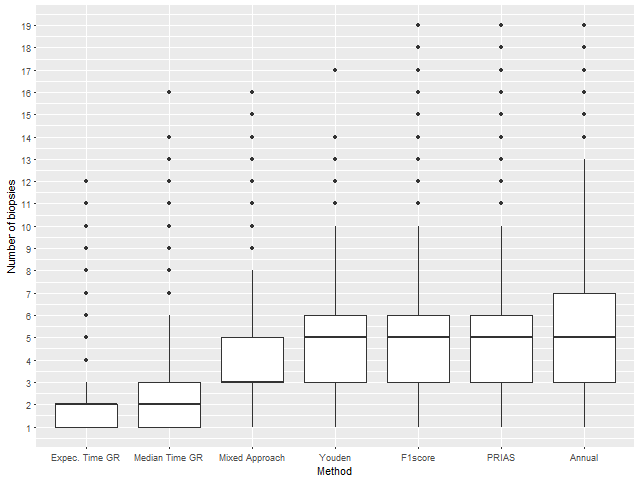
\includegraphics[width=\textwidth]{images/sim_study/nbBoxPlot.png}
        \caption{Boxplot for number of biopsies.}
        \label{fig : nbBoxPlot}
    \end{subfigure}
    \begin{subfigure}[b]{0.45\textwidth}
        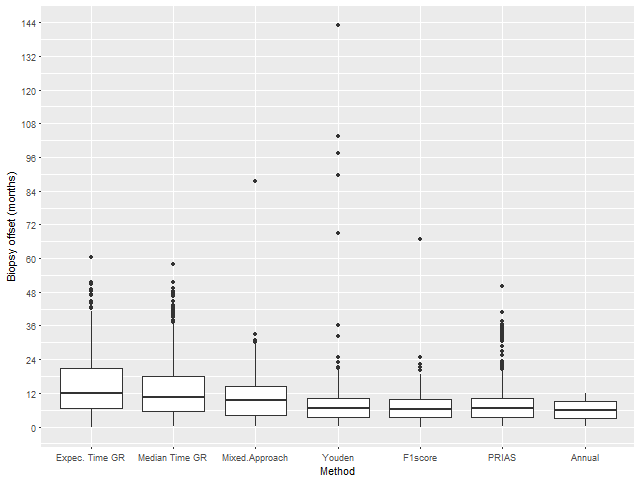
\includegraphics[width=\textwidth]{images/sim_study/offsetBoxPlot.png}
        \caption{Boxplot for offset (months)}
        \label{fig : offsetBoxPlot}
    \end{subfigure}      
    \caption{Boxplot for number of biopsies and offset (months), for all of the 50000 patients in the 200 simulated data sets. Method names are abbreviated for ease of graphing.}
\end{figure}
